% ICEEE 2027, Track 2 (Control Systems, Automation & Computing Technologies)
% IEEEtran conference format, 4-8 double-column pages.
% Build from the repository root with: make pdf
\documentclass[conference]{IEEEtran}

\usepackage{cite}
\usepackage{amsmath,amssymb}
\usepackage{graphicx}
\usepackage{booktabs}

% Figures are copied from dx300-sim by scripts/sync_results.py.
\graphicspath{{../results/}}

\begin{document}

\title{Is Reinforcement Learning Worth It? A Benchmark-Driven Design Study of
Learned Control for an Excavator Boom}

% TODO: confirm author list, affiliation wording and contact line.
\author{\IEEEauthorblockN{Ahmed Ayyad}
\IEEEauthorblockA{Istanbul Okan University}}

\maketitle

\begin{abstract}
% TODO(abstract): write last, after Results is final. No text yet.
% Fed by dx300-sim (paths relative to its root; [synced] = copied to results/):
%   rl/12e_stats.md      [synced]  statistics of the real-plant PID-vs-SAC comparison
%   rl/13_benchmark.*    [synced once it exists]  Lab 13: PPO, TD3, BC, CQL, IQL

\end{abstract}

% TODO: add \begin{IEEEkeywords} ... \end{IEEEkeywords}

\section{Introduction}
% TODO(introduction): no text yet.
% Fed by dx300-sim (paths relative to its root; [synced] = copied to results/):
%   README.md                  study overview, latest result, limitations
%   docs/acceptable_error.md   use case (coarse boom positioning) and tip tolerance
%   docs/12_sac_real_plant.md  design of the learned controller on the real plant


\section{Design Requirements}
% TODO(design requirements): no text yet.
% Fed by dx300-sim (paths relative to its root; [synced] = copied to results/):
%   docs/acceptable_error.md              use case and tip tolerance
%   docs/10_real_plant.md                 real-plant design, source of every value
%   rl/10_real_plant.md                   Lab 10: control study on the real plant
%   rl/10c_dynamic_check.md               Lab 10c: dynamic check against Simscape
%   rl/11_real_plant_tuning.md  [synced]  Lab 11: energy floor, time-limited tuning,
%                                         dump failure
%   rl/11_points.json                     Lab 11 PID operating points


\section{Method Selection}
% TODO(method selection: on/off-policy, online/offline): no text yet.
% Fed by dx300-sim (paths relative to its root; [synced] = copied to results/):
%   docs/12_sac_real_plant.md  Lab 12 design: learned controller on the real plant
%   rl/12_robust_train.py      Lab 12: SAC on the randomized real plant, plain and residual
%   rl/12_sac_train.py         Lab 12b: SAC gain scheduler on the balanced point
%   rl/13_*                    Lab 13 scripts (PPO, TD3, BC, CQL, IQL); not in
%                              dx300-sim yet, list them here once they exist


\section{Benchmark Protocol}
% TODO(benchmark protocol): no text yet.
% Fed by dx300-sim (paths relative to its root; [synced] = copied to results/):
%   rl/12_eval.md                Lab 12 protocol: SAC against the Lab 11 PID points
%   rl/12e_stats.md    [synced]  Lab 12e: statistics of the comparison
%   rl/12_common.py              Lab 12 shared code: controllers, training env, table rows
%   rl/boom_env_real.py          Lab 10a: real plant (Lab 08a Simscape parameters)
%   rl/boom_env_real_robust.py   Lab 12 step 1: robust SAC env on the real plant
%   rl/11_points.json            Lab 11 PID operating points (baselines)
%   rl/13_benchmark.*  [synced once it exists]  Lab 13 protocol


\section{Results}
% TODO(results): no text yet. Take every number from results/, never from memory.
% Fed by dx300-sim (paths relative to its root; [synced] = copied to results/):
%   rl/11_real_plant_tuning.md  [synced]  Lab 11: energy floor and PID points
%   rl/12e_stats.md             [synced]  Lab 12e: statistics of the comparison
%   rl/12f_loads.md             [synced]  Lab 12f: boom cylinder loads per controller
%   rl/12g_sensitivity.md       [synced]  Lab 12g: sensitivity to the estimated plant
%   rl/13_benchmark.*           [synced once it exists]  Lab 13: PPO, TD3, BC, CQL, IQL
%   rl/12d_wsweep.md                      Lab 12d: energy-weight sweep of residual SAC
%   rl/12h_long.md                        Lab 12h: longer SAC training
% Candidate figures, not in the sync list yet (add to SOURCES in
% scripts/sync_results.py when chosen):
%   rl/11_pareto.png, rl/12b_pareto.png, rl/12d_wsweep.png, rl/12h_long.png


\section{Why Learning Lost and When It Would Win}
% Section VI. Why learning lost and when it would win. Full draft from Lab 13,
% with the Lab 14 results in subsection C and the Lab 13e energy split in the limits.
%
% Rule: every number is copied from a file in results/ (synced from dx300-sim,
% commit in results/SOURCE.md). The comment at the end of a line names the file
% and the place in it for the numbers on that line. Nothing is from memory.
% Open items are marked [MISSING: ...] and [CITE: ...] in the text.
%
% Fed by dx300-sim (paths relative to its root; all synced to results/):
%   rl/13_benchmark.md, rl/13_benchmark.csv   Lab 13, table 13d and its reading
%   paper/figs/lab13/fig4, fig5 *.pdf         Fig. 4 and Fig. 5
%   rl/12g_sensitivity.md                     Lab 12g: does the ranking survive plant error
%   rl/12e_stats.md                           Lab 12e: how the PID points were tuned
%   rl/boom_env_real_robust.py                training env of every learner: the reward
%   paper/figs/lab13/README.md                limits of Fig. 4 and Fig. 5 (results/README.md)
%   rl/14_reward_fix.md, rl/14_benchmark.csv  Lab 14: corrected reward, Table II, reward hacking, BC
%   rl/13e_direction_split.md                 Lab 13e: boom-up / boom-down split of E_mech
% Not used here, still candidates: rl/12f_loads.md (its header says "Study, not
% in the paper"), rl/12d_wsweep.md, rl/12h_long.md.

\label{sec:why}%
Section~\ref{sec:results} shows that learning lost. This section asks why, with diagnostics
from the same 7200 moves, and then states the conditions under which the result
could turn. The cause is not the same for the online and the offline learners.

\subsection{Online learners waste energy through command oscillation}

We measure the activity of a controller as the mean absolute rate of the
applied valve command per move, mean $|du/dt|$. % results/13_benchmark.md, definition above table 13d
We split the energy above the floor into oscillation, overshoot and direct
excess. The shares do not add to 100~\% because of a shortfall term. % results/13_benchmark.md, text above table 13d

The economical PID has a command activity of 0.50~s$^{-1}$ and the balanced PID
of 0.64~s$^{-1}$. % results/13_benchmark.md, 13d, rows "economical PID" and "balanced PID"
The online learners move the valve far more: TD3 2.23, SAC 2.81 and PPO
15.96~s$^{-1}$ at the equal budget, which is 4 to 32 times the activity of the
economical PID. % results/13_benchmark.md, 13d, column "mean abs(du/dt) 1/s" and first bullet of the reading
Their energy above the floor is 51.7 to 186.1~kJ per move, against 26.6~kJ for
the economical PID, and 55 to 70~\% of it is oscillation. % results/13_benchmark.md, 13d, columns "excess kJ" and "oscillation %", first bullet of the reading
Fig.~\ref{fig:oscillation} shows the relation for all nine controllers. The
order of the controllers by command activity is also their order by
oscillation energy. % results/13_benchmark.csv, columns du_dt and excess_kJ x oscillation_share / 100 (what Fig. 4 plots); order checked for all 9 rows

This explains the energy result of Section~\ref{sec:results}. An online learner adds a
residual to a PID that is already smooth. The reward penalises tracking error,
speed and power, and has no term on the rate of the command. % results/boom_env_real_robust.py, docstring line "reward" and the reward line in step(): terms e^2, omega^2 and power, none on the command rate; check against Section IV when it is written
The residual that comes out of training switches the valve back and forth, and
the plant turns each reversal into energy that does no useful work on the
boom [CITE: action smoothness in learned continuous control].

The oscillation also explains the accuracy result. The error of the online
learners does not come from the sensor noise. Without noise it is already 5.5
to 14.2~cm, against 1.4~cm for the economical PID. % results/13_benchmark.md, 13d, column "error cm, noise 0 deg", second bullet of the reading
From no noise to 1~deg of noise it changes by 0.8~cm at most, while the error
of the economical PID grows by 2.6~cm. % results/13_benchmark.md, second bullet of the reading under table 13d
The residual itself moves the boom off the target.

More training reduces the oscillation but does not remove it. With about ten
times the environment steps, the command activity of PPO falls from 15.96 to
4.75~s$^{-1}$ and its energy above the floor from 186.1 to 83.7~kJ. % results/13_benchmark.md, 13d, rows "PPO 100k" and "PPO 1M (not equal budget)"
This is still about three times the energy above the floor of the economical
PID. % results/13_benchmark.md, 13d: 83.7 kJ against 26.6 kJ

\begin{figure}[t]
\centering
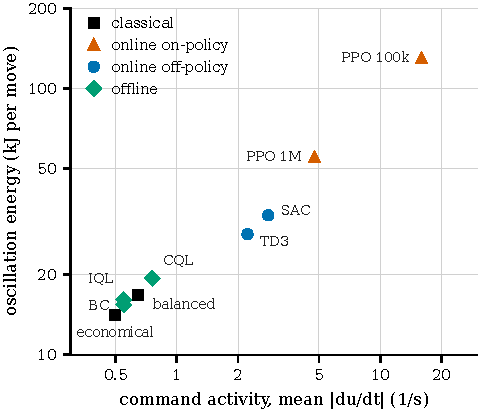
\includegraphics[width=\columnwidth]{fig4_smoothness_vs_oscillation}
\caption{Oscillation energy per move against command activity, both axes
logarithmic. Values pooled over the 3 seeds. Offline learners at 1M
transitions. The fast PID is not shown: its energy split was not computed.} % results/README.md, section "Limits of the figures", item "Fig. 4 has no fast PID"
\label{fig:oscillation}
\end{figure}

\subsection{Offline learners return the dataset}

BC and IQL do not oscillate. Their command activity is 0.55~s$^{-1}$, the level
of the two PID points, and their energy above the floor is 30.0 and 31.6~kJ. % results/13_benchmark.md, 13d, rows "BC, 1M transitions" and "IQL, 1M transitions"
They lose for a different reason. The dataset holds the balanced and the
economical PID in equal parts, and a learner that imitates this mix lands
between the two. This is what Section~\ref{sec:results} shows: 162.6 and 164.1~kJ, between
159.1 and 167.5~kJ. % results/13_benchmark.md, third and fourth bullet of the reading under table 13d
An imitating learner can match the better behaviour in its data. It has no
reason to pass it [CITE: behaviour cloning and its dependence on data quality].
IQL is allowed to weight the data by value [CITE: IQL], but the reward does not
point it to the economical half (Section~\ref{sec:reward}).

CQL fails in a third way. Its command is smooth, 0.76~s$^{-1}$, but its error
is 7.6~cm without any sensor noise, and 56~\% of its 58.2~kJ above the floor is
overshoot. % results/13_benchmark.md, 13d, row "CQL, 1M transitions" and fifth bullet of the reading
CQL ran with the library defaults and on one dataset size, so this is a result
for that configuration and not for the method [CITE: CQL]. % results/13_benchmark.md, section "Setup"

\subsection{The reward does not ask for the economical PID}
\label{sec:reward}

The benchmark ranks the economical PID first on energy: 20.0~\% above the
floor, against 26.4~\% for the balanced PID. % results/13_benchmark.md, 13c, column "gap to floor %"
The training reward ranks the two the other way. On 300 episodes of the
training distribution without noise, the return per episode is $-9.78$ for the
balanced PID and $-10.30$ for the economical PID. % results/13_benchmark.md, last bullet of the reading under table 13d
The 1M dataset, with command noise, gives the same order: $-10.22$ against
$-10.41$, on different episodes for the two behaviours. % results/13_benchmark.md, last bullet of the reading under table 13d; table "Offline dataset", rows 1M
Fig.~\ref{fig:reward_mismatch} shows this pair. A learner that maximises this
reward is not pushed toward the economical PID. With the energy weight
$w = 0.03$, the reward buys the accuracy of the balanced PID with energy, and
the benchmark then counts that energy against the learner.

The evidence has limits. The mismatch is measured for the two PID points only.
The return of the learned controllers that were evaluated was not measured. % results/13_benchmark.md, last bullet of the reading under table 13d
The hollow markers in Fig.~\ref{fig:reward_mismatch} are returns logged during
training, with exploration noise and on the training distribution, so they
give a rough position only. The offline learners have no return and are not in
the figure. % results/README.md, section "Limits of the figures", item "Fig. 5 mixes three kinds of return"
The mismatch is therefore a property of the reward that we have measured. It
is not yet a cause that we have shown.

Lab 14 tests the cause directly. The corrected reward raises the weight of the
power term from 0.03 to 20 and adds a stall term that charges a tip error over
5~cm while the boom is nearly at rest, $|\omega| < 0.01$~rad/s; the sum is
scaled by 1/50. % results/14_reward_fix.md, section "14a. Corrected reward" (both reward lines) and "Status of the values"
SAC and TD3 were retrained on it for 100k environment steps, and IQL and CQL on
the Lab 13 1M dataset relabelled with it. BC was trained on the
economical-PID episodes of that dataset only (500k transitions). % results/14_reward_fix.md, section "Setup"
% Passage a) (approved wording). Returns: results/14_reward_fix.md, table "Return on the training objective"
% (economical -4.699, balanced -4.732, fast -4.830; SAC -4.339, TD3 -4.213). Stop distance and speed: table
% under "Why SAC and TD3 score higher ..." (final error 50.1 / 41.6 cm, mean abs(omega) last 2 s 0.0209 / 0.0212
% rad/s) and table "14e" (mean error 43.0 / 40.6 cm). What the check tested: last bullet of that section.
The corrected reward was checked to rank the economical PID above the balanced
and fast PIDs and above controllers that stop short at rest; SAC and TD3
nevertheless reached a higher return by stopping 40--50~cm short while still
moving above the 0.01~rad/s stall threshold, a behaviour the check did not
include. A reward validated on a finite set of candidate behaviours can still
be exploited by behaviours the optimiser discovers.

Table~\ref{tab:lab14} gives the outcome on the 7200 unseen moves. No Lab~14
controller beats the economical PID. % results/14_reward_fix.md, table "14e", column "beats economical PID", and section "Statement"
SAC and TD3 use less energy than the PID, 136.0 and 134.8~kJ, because they do
not finish the move: 48.06 and 48.75~\% of their moves miss by over 20~cm. % results/14_reward_fix.md, table "14e", rows "SAC 100k, corrected reward" and "TD3 100k, corrected reward"
Learning rates of 0.3 and 3 times the default, one seed each, give 30.22 to
52.82~\% of moves over 20~cm. % results/14_reward_fix.md, table "14e", four rows "lr x0.3 (1 seed)" / "lr x3 (1 seed)", column "miss > 20 cm %"
IQL reaches the energy of the PID, 159.1~kJ, but not its accuracy: 3.1~cm mean
error and 0.47~\% of moves over 20~cm. CQL still misses 10.62~\%. % results/14_reward_fix.md, table "14e", rows "IQL 1M, corrected reward" and "CQL 1M, corrected reward"
% Passage b) (approved wording; 2.2 cm per results/14_reward_fix.md, 4.371 - 2.136 cm in results/14_benchmark.csv).
% results/14_reward_fix.md, table "14e", rows "economical PID" and "BC, economical-PID data only (500k)";
% p: column "median diff error cm (p)"; gap: table "Does the gap close?" and bullet "Data (14c)".
BC trained on economical-PID data is 1.5~kJ cheaper (157.6 vs 159.1~kJ) but
2.2~cm less accurate (4.4 vs 2.1~cm mean error), with 0.1~\% vs 0~\% misses
(paired test $p < 10^{-300}$); it does not beat the PID on both accuracy and
energy.
A reward that ranks the PID points in the intended order was not enough to
close the gap. % results/14_reward_fix.md, section "Statement", last bullet

\begin{table*}[t]
\centering
\caption{Lab 14 benchmark on the 7200 unseen moves of Table~\ref{tab:benchmark}
(simulation). Learners retrained with the corrected reward; BC trained on the
economical-PID data only. Mean $\pm$ standard deviation over 3 seeds unless
noted. No controller beats the economical PID.}
\label{tab:lab14}
\footnotesize
% Every row: results/14_reward_fix.md, table "14e. All controllers against the economical PID"
% (full precision: results/14_benchmark.csv). Budgets: results/14_reward_fix.md, section "Setup".
\begin{tabular}{@{}llccccccc@{}}
\toprule
Controller & Training budget & Miss $>$10 cm & Miss $>$20 cm & Mean error & P95 error
  & $E_{\mathrm{mech}}$ & Gap to floor$^{\mathrm{a}}$ & Beats the \\
 & & (\%) & (\%) & (cm) & (cm) & (kJ) & (\%) & econ.\ PID \\
\midrule
Economical PID & none & 0.97 & 0.00 & 2.1 & 6.4 & 159.1 & 20.0 & -- \\ % results/14_reward_fix.md, 14e, row "economical PID"
\midrule
\multicolumn{9}{@{}l}{\emph{Online, off-policy, corrected reward}} \\
SAC & 100k steps & $66.82 \pm 8.94$ & $48.06 \pm 8.30$ & $43.0 \pm 12.4$ & $164.8 \pm 42.5$ & $136.0 \pm 9.8$ & $2.6 \pm 7.4$ & no \\ % results/14_reward_fix.md, 14e, row "SAC 100k, corrected reward"
TD3 & 100k steps & $66.36 \pm 4.78$ & $48.75 \pm 9.73$ & $40.6 \pm 12.3$ & $141.0 \pm 19.4$ & $134.8 \pm 9.0$ & $1.7 \pm 6.8$ & no \\ % results/14_reward_fix.md, 14e, row "TD3 100k, corrected reward"
\midrule
\multicolumn{9}{@{}l}{\emph{Offline; IQL and CQL: corrected reward, Lab 13 dataset relabelled}} \\
IQL & 1M transitions & $4.73 \pm 6.16$ & $0.47 \pm 0.72$ & $3.1 \pm 1.2$ & $9.3 \pm 4.2$ & $159.1 \pm 0.2$ & $20.1 \pm 0.2$ & no \\ % results/14_reward_fix.md, 14e, row "IQL 1M, corrected reward"
CQL & 1M transitions & $33.88 \pm 31.88$ & $10.62 \pm 14.28$ & $8.8 \pm 5.9$ & $21.4 \pm 12.4$ & $150.5 \pm 3.7$ & $13.6 \pm 2.8$ & no \\ % results/14_reward_fix.md, 14e, row "CQL 1M, corrected reward"
BC, econ.\ PID data & 500k transitions & $5.62 \pm 2.65$ & $0.09 \pm 0.08$ & $4.4 \pm 1.4$ & $9.8 \pm 1.7$ & $157.6 \pm 0.9$ & $18.9 \pm 0.7$ & no \\ % results/14_reward_fix.md, 14e, row "BC, economical-PID data only (500k)"
\midrule
\multicolumn{9}{@{}l}{\emph{Learning-rate check, corrected reward, 1 seed}} \\
SAC, lr $\times 0.3$ & 100k steps & 68.97 & 52.82 & 40.5 & 145.7 & 134.2 & 1.2 & no \\ % results/14_reward_fix.md, 14e, row "SAC 100k, corrected reward, lr x0.3 (1 seed)"
SAC, lr $\times 3$ & 100k steps & 45.67 & 30.22 & 36.3 & 187.4 & 132.1 & $-0.3$ & no \\ % results/14_reward_fix.md, 14e, row "SAC 100k, corrected reward, lr x3 (1 seed)"
TD3, lr $\times 0.3$ & 100k steps & 67.00 & 45.28 & 32.5 & 122.1 & 139.3 & 5.1 & no \\ % results/14_reward_fix.md, 14e, row "TD3 100k, corrected reward, lr x0.3 (1 seed)"
TD3, lr $\times 3$ & 100k steps & 59.69 & 33.83 & 26.6 & 83.5 & 143.9 & 8.6 & no \\ % results/14_reward_fix.md, 14e, row "TD3 100k, corrected reward, lr x3 (1 seed)"
\bottomrule
\multicolumn{9}{@{}l}{$^{\mathrm{a}}$The floor is the least energy of the full move. A controller that does not finish the move can come close to it or below it.} \\ % results/14_reward_fix.md, note under table "Command smoothness and energy split"
\end{tabular}
\end{table*}

\begin{figure}[t]
\centering
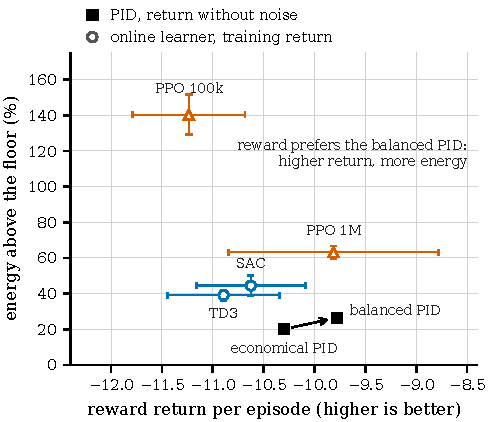
\includegraphics[width=\columnwidth]{fig5_reward_mismatch}
\caption{Energy above the floor against the return of the training reward.
Filled squares: PID points, return without noise on the training distribution.
Hollow markers: online learners, return logged during training (rough position
only). The energy axis is from the unseen evaluation moves. The reward gives
the balanced PID the higher return although it uses more energy.}
\label{fig:reward_mismatch}
\end{figure}

\subsection{When learning would win}

The result is negative for this testbed and this setup. The diagnostics point
to the conditions that would have to change. We state them as conditions, not
as results.

\emph{The reward must rank controllers as the benchmark does.} A learner
cannot be expected to find an operating point that its objective scores below
another one. This is the condition that Lab 14 tests.
% Passage c) (approved wording). results/14_reward_fix.md, table "14e", rows "SAC 100k, corrected reward"
% (136.0 kJ, 48.06 % miss > 20 cm) and "economical PID" (159.1 kJ, 0.00 %); last bullet of "Statement".
% No citation for Lagrangian SAC yet: add one from refs.bib before submission.
Lab 14 shows that a reward penalty for misses can be traded against energy
(SAC 136.0~kJ at 48.1~\% misses vs PID 159.1~kJ at 0~\%); a hard accuracy
constraint (e.g.\ Lagrangian SAC) removes that trade and is the natural next
step. It requires its own cost-threshold tuning and full evaluation, and is
left for future work.

\emph{The command must be kept smooth.} The online learners lose their energy
to oscillation, not to a wrong operating point. A penalty on the command rate,
a filter on the action or a policy with a smoothness constraint attacks this
cause directly [CITE: action smoothness in learned continuous control]. We did
not test any of these.

\emph{The data must contain something better than the baseline.} BC and IQL
return what the dataset holds. Here the dataset was made by the two PID points,
so the economical PID is the best that imitation can reach. Offline learning
can only win with data from a better source, or with a method that reliably
improves on its data [CITE: offline RL and dataset coverage].

\emph{The baseline must be weak or expensive.} The PID points needed no
training. They were tuned by a grid search on 20 tuning scenarios. % results/12e_stats.md, section "Training cost"
Every learned controller needed at least 100k environment steps or a dataset of
100k transitions, and still lost. % results/13_benchmark.md, table 13c and table "Dataset size (offline)"
Learning is more likely to pay where no such baseline exists, for example in
coordinated multi-joint motion or in contact with soil [CITE: learned control
of excavators beyond single-joint tracking]. A single-joint boom testbed cannot
show this.

Plant error alone is not such a condition. In Lab 12g we perturbed the moment
arm, the gravity torque, the inertia and the cylinder friction of the plant by
factors of 0.8 to 1.2, while the controllers kept the nominal model. % results/12g_sensitivity.md, header
The economical PID dominated all four SAC variants of Lab 12 in 31 of the 33
plant settings. % results/12g_sensitivity.md, section "Summary"
In the other two settings, with the moment arm, the gravity torque and the
inertia all 20~\% above nominal, one SAC variant used less energy than the PID
(188.1 against 191.5~kJ, and 188.0 against 191.1~kJ). It still missed 4.42~\%
and 4.46~\% of the moves by over 20~cm, against none for the PID. % results/12g_sensitivity.md, table "Per setting", rows r1.2_g1.2_j1.2_b0.8 and r1.2_g1.2_j1.2_b1.2, columns "PID economical" and "res_eco_w0.1"
This test covers SAC only.

Two limits bound all of these statements. First, the testbed is a
single-joint boom model with estimated geometry, and there is no real-machine
data. Second, the Lab 13 learners ran close to their library defaults, with
3 seeds and one energy weight, while the PID points were tuned on the testbed. % results/13_benchmark.md, section "Setup"; results/12e_stats.md, section "Training cost"
A tuned learner may do better than the ones we report. The benchmark shows
that learning lost under these conditions. It does not show that learning must lose.

% Passage d) (approved wording). results/13e_direction_split.md, table "Per controller" (16 rows, Lab 13
% controllers only; columns "boom-down %" 45.06-48.62 and "W_neg %" 42.67-45.41, means over seeds)
% and section "Spread" (3.56 percentage points).
Across all 16 Lab~13 controllers, 45.1--48.6~\% of mechanical work is spent
lowering the boom and 42.7--45.4~\% is negative work; the lowering share
differs by at most 3.6 percentage points. Errors in the boom-down model, the
least validated part of the plant, therefore affect all controllers similarly;
we compare controllers relative to each other and do not claim the absolute
lowering energy.


\section{Design Lessons}
% TODO(design lessons): no text yet.
% Fed by dx300-sim (paths relative to its root; [synced] = copied to results/):
%   README.md                             Method and Limitations sections
%   rl/11_real_plant_tuning.md  [synced]  Lab 11: energy floor and PID points
%   rl/12e_stats.md             [synced]  Lab 12e: statistics of the comparison
%   rl/12g_sensitivity.md       [synced]  Lab 12g: sensitivity to the estimated plant
%   rl/13_benchmark.*           [synced once it exists]  Lab 13: PPO, TD3, BC, CQL, IQL


\section{Conclusion}
% TODO(conclusion): write after Results and Design Lessons. No text yet.
% Fed by dx300-sim (paths relative to its root; [synced] = copied to results/):
%   rl/12e_stats.md    [synced]  Lab 12e: statistics of the comparison
%   rl/13_benchmark.*  [synced once it exists]  Lab 13: PPO, TD3, BC, CQL, IQL
%   README.md                    Limitations and Roadmap sections


% TODO: uncomment the two lines below at the first \cite. With no citation in
% the document BibTeX writes an empty reference list and the build fails.
% \bibliographystyle{IEEEtran}
% \bibliography{refs}

\end{document}
